\documentclass[conference]{IEEEtran}

\usepackage{cite}
\usepackage[dvips]{graphicx}
\usepackage[cmex10]{amsmath}
\interdisplaylinepenalty=2500
\usepackage{array}
\usepackage[tight,footnotesize]{subfigure}

% correct bad hyphenation here
\hyphenation{op-tical net-works semi-conduc-tor}

\begin{document}

\title{Energy-Conscious Prototype for Enabling Multi-Protocol Wireless Communications}


\author{\IEEEauthorblockN{Travis~Collins\IEEEauthorrefmark{1}, Patrick~DeSantis\IEEEauthorrefmark{1}, David~Vecchiarelli\IEEEauthorrefmark{1}, Alexander~M.~Wyglinski\IEEEauthorrefmark{1}, and Sean~McGrath\IEEEauthorrefmark{2}\\ \\}
\IEEEauthorblockA{\IEEEauthorrefmark{1}Wireless Innovation Laboratory\\
Department of Electrical and Computer Engineering\\
Worcester Polytechnic Institute, Worcester, MA 01609--2280, USA\\
Email: \{traviscollins,~pdesantis,~davevecc,~alexw\}@wpi.edu\\ \\}
\IEEEauthorblockA{\IEEEauthorrefmark{2}Wireless Access Research Centre\\
Department of Electronic and Computer Engineering\\
University of Limerick, Limerick, Ireland\\
Email: sean.mcgrath@ul.ie}}


% make the title area
\maketitle


\begin{abstract}
In this paper, we present a novel hardware prototype implementation
of a wireless communication system capable of automatically
selecting one of several available commercial standards in order to
minimize energy utilization while simultaneously achieving
reasonable data rate performance.  Without loss in generality, two
wireless standards were employed in the prototype implementation,
namely: ZigBee and WiFi.  These standards were chosen due to their
complementary characteristics with respect to data bandwidth and
energy efficiency.  At the core of the prototype implementation is a
{\it decision-making module} designed to automatically select the
most suitable wireless standard for data transmission based on the
instantaneous network load and the operating conditions of the
wireless platform, such as battery life.  The prototype
implementation was evaluated across several data transmission
scenarios, including file transfers, web browsing, streaming media
and text messaging.  By leveraging the concepts of sensing and
adaptation often employed in {\it cognitive radio}, the prototype
system monitors and selects the lowest power intensive wireless
protocol while still maintaining an acceptable quality of service
for the desired application.  Even though performance transparency
could not be sacrificed for power efficiency, experimental
validation of this network design shows substantial energy savings:
more than a 30\% reduction in energy consumption of the wireless
interfaces is possible, leading to a substantial increase in the
effective battery lifetime of a energy-limited wireless networking
device.
\end{abstract}



\section{Introduction}

Modern society's usage of wireless communication devices is growing
at an exponentially increasing rate, driven primarily by the
cellular telephony and mobile computing markets~\cite{two}. However,
this growth comes at the expense of global energy consumption used
to enable these devices and the infrastructure used to support them.
According to~\cite{three}, it was stated that ``currently 3\% of the
world-wide energy is consumed by the ICT (Information \&
Communications Technology) infrastructure that causes about 2\% of
the world-wide CO2 emissions, which is comparable to the world-wide
CO2 emissions by airplanes or one quarter of the world-wide CO2
emissions by cars.''  Consequently, given this level of energy
consumption and its associated impact on the environment, coupled
with minimal advances in the battery technology sector~\cite{five},
has made energy efficiency and power saving strategies an
increasingly important design requirement for modern wireless
devices.
\begin{figure}[t]
\begin{center}
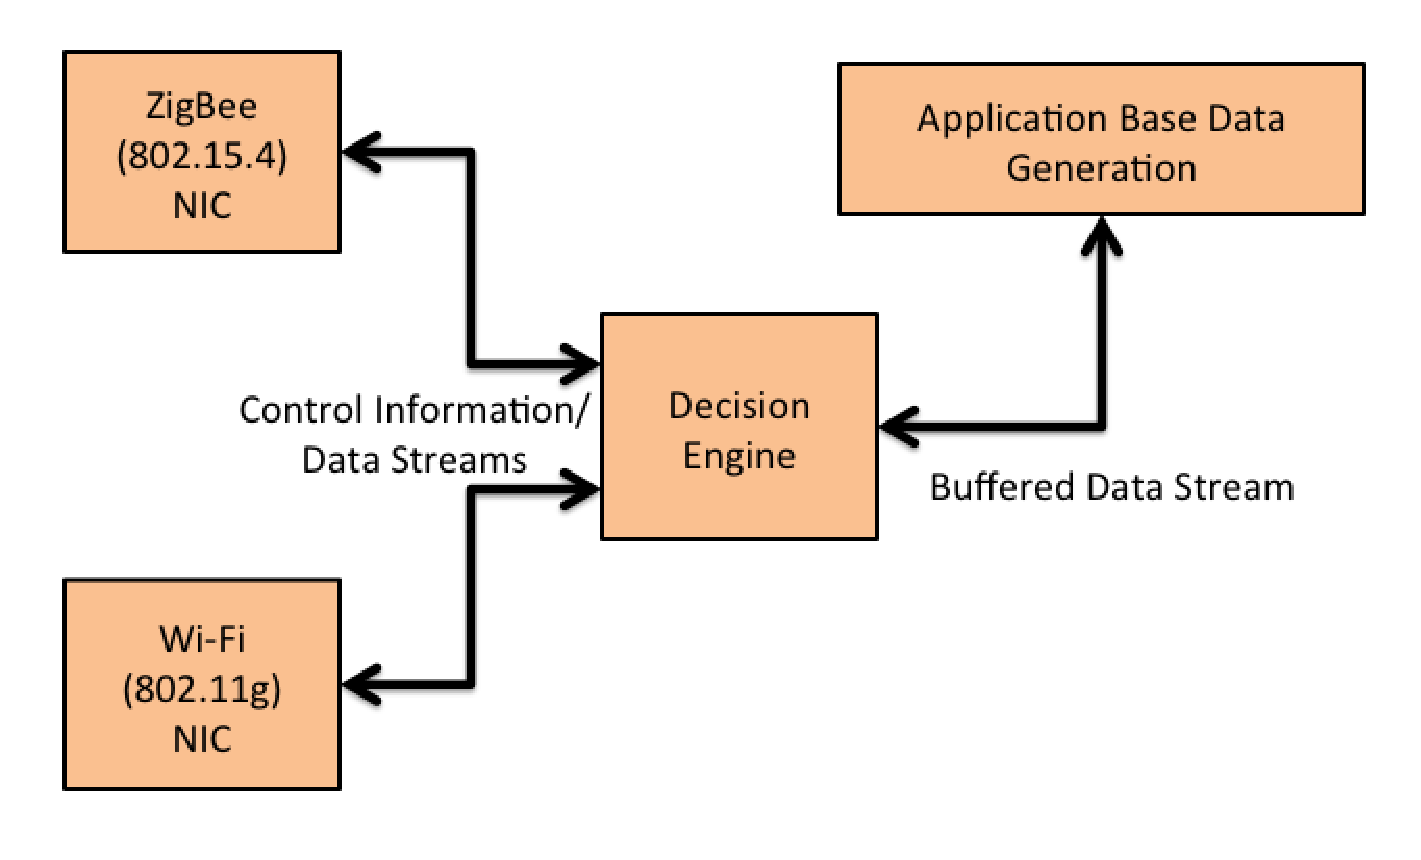
\includegraphics[scale=0.35]{concept_diagram.eps}
\caption{System concept diagram of the proposed energy-conscious
prototype implementation, showing how network traffic is filtered by
a decision-making engine in order to decide which
networking interface should be employed at both the transmitter and
receiver modules. The two networking interfaces shown here are
ZigBee (IEEE~802.15.4) and Wi-Fi (IEEE~802.11g).}
\end{center}\label{f:concept}
\end{figure}

With the rapidly growing adoption of smart~phones, laptops,
netbooks, and portable tablet computers by modern society, the
ability for a wireless mobile device to save power in order to
extend its battery life has been a very active area of research and
development by both industry and academia. In terms of reducing
wireless communications power consumption, one approach that can be
employed is to utilize multiple wireless protocols in order to
achieve some degree of power savings while still maintaining an
acceptable level of data bandwidth for performing mobile tasks. Many
mobile devices support several wireless protocols, such as Wi-Fi,
Bluetooth, and 3G.  In~\cite{six}, the benefits of such a combined
protocol network was investigated.  Specifically, two networking
standards were employed by a single wireless system, namely,
Bluetooth and Wi-Fi. The actual prototype used complex switching
intelligence and the advantages of using a multiprotocol network and
important switching characteristics were examined.  Furthermore,
several switching policies were studied in order to assess whether
power saving methods can be realized via the reduction of Wi-Fi
activity. The policies used several measurement techniques, such as
received signal strength indicator (RSSI) metrics, transmit power,
link quality, and bandwidth capacity.  These measurements were
obtained in order to determine the appropriate switching times
between wireless protocols~\cite{six}. Bandwidth was the primary
metric for the switching calculations performed in~\cite{six}.
Although several of the techniques proved to be unsuccessful, power
savings were realized but at the price of mobility.  The primary
issue with this design was the use of Bluetooth technology.

In practice, Bluetooth is not a suitable choice for mobile
applications due to its limited transmission range. Rather,
Bluetooth was developed as a cable replacement protocol and not for
multiuser mobility.  For this reason, Bluetooth has a very short
transmission range making it much less effective relative to other
low-power wireless access technologies~\cite{thirteen}. With an
infrastructure based network, Bluetooth provides insufficient
mobility and thus seriously limits users or vastly increases the
need for additional access points. In this paper, we implement a
hardware prototype system designed to minimize power consumption and
achieve a reasonable level of data bandwidth on demand by
automatically switching between the power efficient, low data rate
wireless data transmission standard called ZigBee and the high
power, high data rate wireless data transmission standard referred
to as Wi-Fi.  These protocols will be controlled through an onboard
algorithm that monitors the bandwidth of a wireless network,
reacting to increases and decreases in network activity, deciding
when to switch between protocols. The algorithm monitors the
bandwidth of the active wireless systems, and correlates
predetermined power consumption to that usage, which was obtained
via pre-profiling the communication interfaces.  Thus, when the
wireless network requires more capacity, the algorithm selects the
Wi-Fi interface for data transmission/reception, and when little to
no data capacity is needed the algorithm selects the ZigBee
interface.  Intuitively, this dual protocol switching approach
possesses a power advantage due to the generally limited amount of
network activity of mobile devices compared with the duration of
their uptime. This design overcomes the shortcomings of current
single protocol networks by:
\begin{enumerate}
  \item  Alternating between two complementary wireless standards without sacrificing mobility and throughput, and decreasing communications power consumption over time.
  \item  Intelligently monitoring the bandwidth of multiple radios directly and reactsing to changes in the bandwidth.
  \item  Being power consumption aware by making decisions as well as alternating automatically based on power consumption, bandwidth needs, battery level,
  etc.
\end{enumerate}

The rest of this paper is organized as follows: In Section~II, we
present the overall proposed communication system, while in
Section~III we describe the power profiling process of the
communication interfaces as well as the implemented hardware
prototype system.  In Section~IV, the actual experiments with the
hardware prototype and the experimental results are presented, and
several concluding remarks are drawn in Section~V.


\section{Proposed Communication System}
The concept diagram for the proposed prototype system is shown in
Fig.~\ref{f:concept}.  The prototype implementation uses a hybrid
Wi-Fi and ZigBee interface in order to provide improved power
efficiency for mobile devices while not sacrificing data bandwidth
requirements. Thus, from a network perspective, each node in the
network can be equipped with both a ZigBee and a Wi-Fi radio
interface such that the appropriate interface can be selected by a
decision-making algorithm running onboard the system.  Based on the
idle power consumption of typical Wi-Fi and ZigBee radios (see
Table~\ref{t:table1}), this concept has the potential to realize a
large reduction in power consumption for an idle system.  However,
the actual power savings heavily depends on the switching
characteristics. The proposed implementation uses commercially
available networking interfaces and thus does not require any
significant hardware changes. A ZigBee interface, which already
exists in many commercial mobile devices, was installed. ZigBee is a
low-power and low-cost interface, making it relatively inexpensive
to install on many current mobile devices, such as cellular
telephones. \setcounter{table}{0}
\begin{table}[t]
\caption{A Comparison of Wireless Standards Employed in Most Modern
Mobile Wireless Devices~\cite{eight,six,nine,ten,eleven,fourteen}.}
\begin{center}
\begin{tabular}{llll}
\hline
Qualifier & Wi-Fi & ZigBee\\
\hline
Data Rate & 54 Mb/s & 250Kb/s\\
Transmission Power Draw & 32-100mW & 0.001-.003mW\\
Idle Power Draw & 0.085W & 0.001-.003mW\\
\hline
\end{tabular}
\end{center}
\label{t:table1}
\end{table}

\section{Prototype Implementation}
\subsection{System Architecture}
The experimental prototype is designed to evaluate the performance
of the proposed communication system as well as single protocol
communication devices across a range of network applications. The
network topology was designed to infrastructure-based, which is a
mode of operation that is generally employed more often by
Internet-ready wireless devices.  Without loss in generality, the
prototype implementation will only utilize two nodes, a mobile user
and a base station or router. All power savings and adaptive
protocol switching will focus on the mobile user. Since it is
assumed that the base station will operate using a stable power
source, its energy consumption will be neglected in this research.
\begin{figure}[t]
\begin{center}
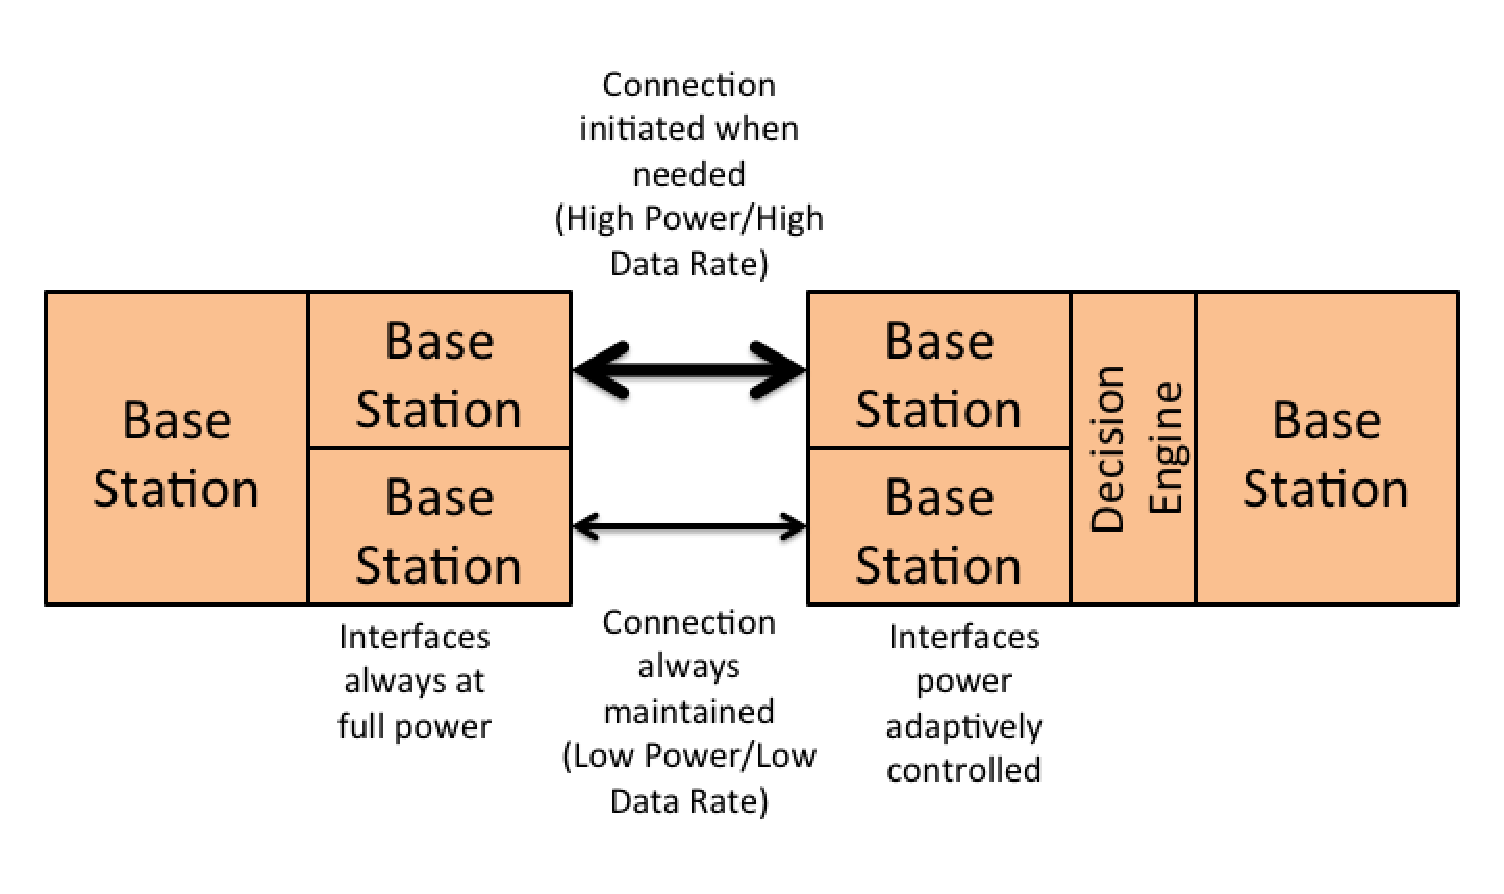
\includegraphics[scale=0.35]{system_diagram.eps}
\caption{A system diagram of the prototype implementation setup with
both external networking interfaces being monitored in real-time.
Both wireless networking interfaces are monitored directly to
provide direct information about power consumption, and allow for
evaluation of the switching intelligence of the mobile user.}
\end{center}
\end{figure}

Data for the network is generated in order to represent typical
Internet usage for a given duration.  This data is then buffered
into a single queue, as seen from Fig.~\ref{f:concept}, then the
switching engine determines which interface will transmit this data.
At all times, the ZigBee connection will be maintained and Wi-Fi
will be initiated through the transmission of ZigBee control packets
when additional bandwidth is demanded.  Since bandwidth can be
relatively difficult to measure from two independent interfaces
quickly, the data queue is used instead to measure the bandwidth.
Based data queue characteristics, relative data rates can be
determined.

The tests performed by the mobile user represent common applications
performed by mobile devices such as smart~phones.  The four
applications examined in this work were: large file transfers, small
file transfers, web browsing, and purely idle utilization.  All
relevant data was captured by a third data acquisition computer
workstation. From this workstation, the data is viewed graphically
in real-time and exported to a file for analysis.

The ZigBee interface was the most challenging to construct due to
the limited sophistication of the selected modules.  A relatively
simple version of TCP was built upon the open-source API
xbee-api~\cite{fifteen}.  The implementation provided the necessary
functionality in order to maintain links between the ZigBee modules
and the complete bi-directional file transfers.  This was abstracted
in the devised switching engine in order to simplify the interface.

The switching engine itself dynamically alternates between the
ZigBee and Wi-Fi interfaces by using three primary parameters:
bandwidth, queue size, and power consumption.  Power consumption was
predetermined directly via measurements, and was directly related to
the transmission usage. Therefore, at any given time, the power
consumption could be determined via data bandwidth usage.  This
switching engine not only possessed the ability to direct data flow,
but also to initiate connections of the interfaces and reduce their
overall power as well.  This switching engine was only developed on
the mobile user, the base station or routing unit would remained at
full power on both interfaces at all times.
\begin{figure}[t]
\begin{center}
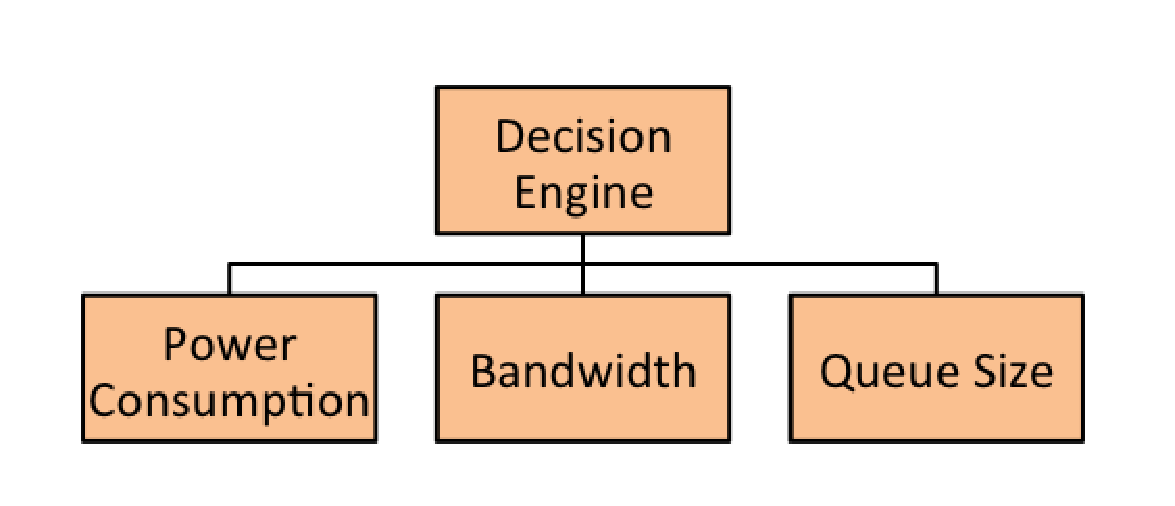
\includegraphics[scale=0.40]{cognitive_para.eps}
\caption{Breakdown of operating parameters for the decision engine
employed in the prototype implementation.}
\end{center}
\end{figure}

The base station device effectively acts as a wireless hub which
supports both ZigBee and Wi-Fi capabilities, keeping both interfaces
active at all times.  The mobile node was responsible for running
all network utilization tests and has both wireless interfaces power
consumption actively monitored. A third data acquisition machine was
originally used for power profiling, and then to measure power usage
during experiments.  It utilized a pair of multimeters in order to
capture detailed power usage of the mobile user.  From this data,
energy was determined of the networking interfaces during transmit,
receive, and idle modes.  These results can be seen in
Table~\ref{t:table2}. \setcounter{table}{2}
\begin{table}[b]
\caption{Wi-Fi and ZigBee Power Consumption Measurements.}
\begin{center}
\begin{tabular}{llll}
\hline
Protocol & Action & Power(W) & STD(W)\\
\hline
ZigBee & Tx (Average) & 0.365 & 0.001\\
ZigBee & Rx (Average) & 0.360 & 0.003\\
Wi-Fi & Tx (Average) & 1.454 & 0.005\\
Wi-Fi & Rx (Average) & 1.402 & 0.006 \\
\hline
\end{tabular}
\end{center}
\label{t:table2}
\end{table}


\subsection{Hardware Components}
The base station and mobile node are virtually identical hardware
components built around the Eee PC 4G Netbook, as shown in
Fig.~\ref{f:prototype}. Each netbook runs a standard version of the
Ubuntu~9.10 operating system. The mobile node uses a Linksys~WUSB54G
wireless interface adapter for Wi-Fi, and a XBee~Series~2~OEM~RF
Module for ZigBee. The Wi-Fi module uses hand compiled drivers based
upon the MadWifi driver. Unless otherwise noted, all Wi-Fi traffic
was performed in constantly active mode (CAM), due to that fact that
only an ad-hoc wireless can could be utilized for direct connections
between netbooks.  Also Wi-Fi connection information is passed
through the always on ZigBee connection to primarily reduce the
association time of Wi-Fi.
\begin{figure}[t]
\begin{center}
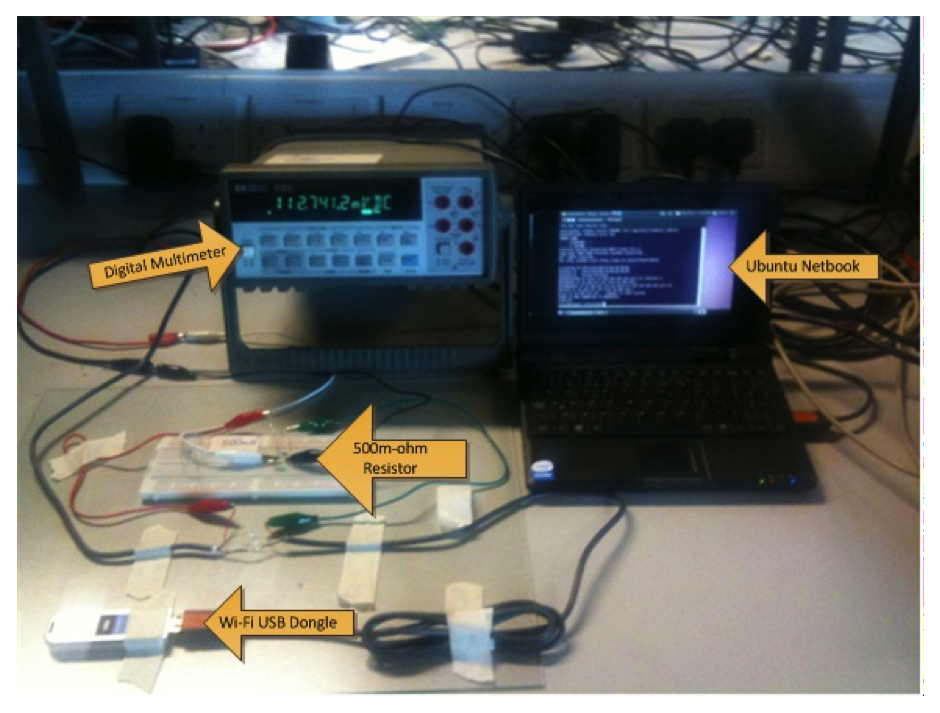
\includegraphics[scale=0.50]{actual_testbench.eps}
\caption{Photograph of the actual hardware prototype implementation
with only a single multimeter, which is being employed in order to
measure the power consumption of the Wi-Fi USB dongle.}
\end{center}\label{f:prototype}
\end{figure}

\subsection{Protocol Alternating}
The basic switching process encompasses a start-up process for the
higher-level radio that incurs some delay.  The initial switching
process can roughly be divided into three parts: connection
initiation request, power-up, and connected.  Since the ZigBee
channel is always available for communication, data transfer
continues until the switch to use the Wi-Fi interface is complete.
Both interfaces are abstracted as a single interface to the
operating system.  Data is first buffered into a queue that leads to
both interfaces.  Then based upon the amount of data in the queue
and how quickly data is added or removed from it determines when to
switch between the interfaces occurs.  This switch causes a switch
in the queue's output interface as well, forcing data either through
only ZigBee or only Wi-Fi.  These thresholds are based upon measured
power characteristics of the physical wireless hardware, the battery
level of the node, and application demand.  Since a design
requirement was performance transparency, most tasks need to use
Wi-Fi to transfer data without considerable delay visible to the
user.  Therefore application demand does trump most switching
decisions.  Wi-Fi association time was highly focused upon to reduce
possible lag during switches.

\section{Experimental Setup}
\subsection{Experimental Results}
Fig.~\ref{f:compare_results1} shows an overview of the benefits
provided by the proposed implementation, compared to a Wi-Fi CAM,
Wi-Fi PSM, and ZigBee showing both energy and time for a variety of
transfer task-base tests. These results represent power consumption
per activity.  It is important to note that for most mobile devices
that greater that 70\% of device uptime is spent is idle mode.
Although dynamic switching the mobile device can remain out of the
power hungry Wi-Fi idle state, and only utilize it when larger data
load become queued. On its own, the ZigBee interface provides the
lowest energy consumption advantage during idle testing, but as soon
as any bandwidth intensive task is performed it becomes very power
inefficient. Wi-Fi is very power efficient when it comes to data
transfer, but when the node becomes idles this is no longer the
case.  The proposed network implementation shines in both these
cases, expect when the Wi-Fi interface must be maintain for more
than 70\% of the device's uptime.  Fortunately for mobile users,
70\% network utilization time is extremely rare.  Overall, when
compared with Wi-Fi, the less time the node is actively transferring
data the more energy is saved with the proposed network
implementation.  The graph below illustrates this fact, extrapolated
from measured result of the implemented hardware.
\begin{figure}[t]
\begin{center}
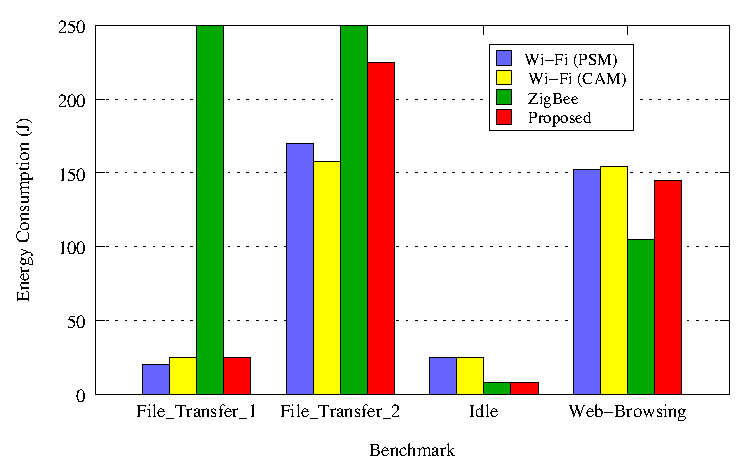
\includegraphics[scale=0.65]{woot.eps}
\caption{Experimental results from the four tests used to evaluate
the performance of ZigBee (Green), Wi-Fi PSM (Red), Wi-Fi CAM
(Blue), and the proposed implementation (Purple).  File transfer 1
(Far left test) examines the power usage of a transfer that last for
25\% of the test duration.  File Transfer 2 (Second from left)
transfers a file for 80\% of the test. The Wikipedia or web-browsing
test (second from right) examines common web-browsing usage across a
60 second interval derived from the IMIX web studies of web-browsing
habits. \cite{twelve}  The final test (far right) examines power
usages for 20 seconds during active no transfers or an idle state.}
\end{center}\label{f:compare_results1}
\end{figure}

Fig.~\ref{f:compare_results2} are the results of a 56\% high demand
transfer test.  The figure illustrates the power savings over time.
Even at such a high data transfer rate a 10\% decrease in overall
power consumption is observed, which as previously explain is an
extremely rare usage percentile.  Extrapolating from this data, a
saving of 53\% can be saved.
\begin{figure}[b]
\begin{center}
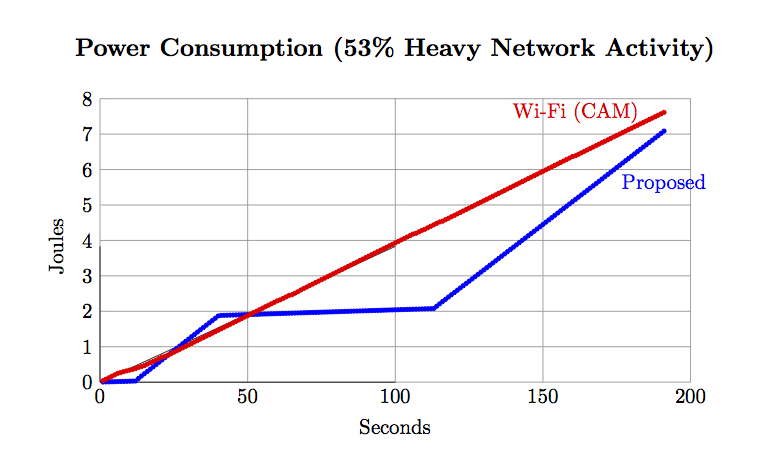
\includegraphics[scale=0.70]{energy_con.eps}
\caption{The above graph compared the amount of energy used over a two minute file transfer test with 53\% activity between a single protocol Wi-Fi (CAM) network and the proposed network.}
\end{center}\label{f:compare_results2}
\end{figure}


\subsection{Power Measurement Strategy}
The energy measurement setup consists of a HP DAQ Multi-meter data
acquisition device connected to a standard Windows XP desktop system
with MATLAB. The individual power rails for Wi-Fi and ZigBee are
monitored by placing separate 1\%-tolerance 500~m$\Omega$ resistors
in series with each subsystem's power supply. Samples are measured
at 500~ms intervals, the maximum speed of the multi-meters.  Energy,
and not power consumption, is used to show the majority of the
results because it captures both the power and time aspects of a
particular benchmark. Other components, such as processor, power
regulators, memory, and display are not included since despite the
fact that they are significant power consumers of the mobile
device's battery, they cannot be easily directly measured
independently.

Since power consumption monitors do not exists on common network
interface cards, it was assumed that direct real-time measurement
and feedback would be impractical.  Therefore a power profile was
determined for each network interface cards.  With this profile
data, at any data-rate the power being consumed could be calculated
in real-time indirectly.  This data was then directly used by our
decision engine to make determinations when to alternate protocols.
This profile was compared with direct measurements during testing to
confirm proper switching and assumed power consumption.


\section{Conclusion}
With an ever-increasing focus of today's world today on mobile data
connectivity, greater efficiency when performing data communications
while using these mobile devices is growing in importance.  The work
presented in this paper is a step in a positive direction with
respect to energy efficient wireless devices. Using off-the-shelf
components highlighted the fact that energy efficient approaches can
be readily realized using today's technology.  Combining the
ubiquity of wireless devices and the ever growing marketplace,
multiprotocol systems show tremendous promise for the future. The
applications for multiprotocol systems are far ranging, from large
scale communication networks, to household appliances and networks.
The greatest advantage is the simplicity of the proposed concept.
The prototype implementation achieved the following goals:
\begin{enumerate}
  \item A Multi-protocol Networking Device:  The system was able to utilize dual radio protocols to transmit data
  synchronously.
  \item Power Efficiency:  The system was able to considerably reduce the communications power consumed compared with a single protocol
  network.
  \item Performance Transparency:  The multiprotocol network performed equally or greater than the a single protocol network as  in terms of
  throughput.
  \item Commercially Available Equipment: This project only utilized off the shelf part in both nodes of the
  network.
\end{enumerate}

By demonstrating the feasibility of this prototype implementation
via practical means, this work has provided a foundation for future
research and development efforts in the area of multiprotocol
systems designed to satisfy both power efficiency and bandwidth
requirements.

\bibliographystyle{IEEEtran}
\bibliography{LPCN_Conference_Paper_refs}


\end{document}
